
\clearpage
\section{Die Adressliste benutzen}
\label{bkm:Ref443738751}
In der Adressliste werden auf einfache Art und Weise sämtliche im CUBE PA erfassten Personen (Benutzer) und Firmen angezeigt. Mittels der Filterfunktion können Einträge rasch gefunden werden.

\vspace{\baselineskip}

Für die Benutzung der Adressliste sind folgende Eigenschaften zu berücksichtigen:

% \liststyleWWviiiNumxiii
\begin{itemize}
\item
Ist ein Benutzer des CUBE PA entsprechend berechtigt, kann er in der Adressliste neue Personen und Firmen erfassen oder bestehende Einträge bearbeiten.

\item
Personen, welche auf diese Weise erfasst wurden, stehen automatisch in allen Personen-Auswahlfeldern zur Verfügung (z.B. Pendenzen). Jedoch können sich diese neu erfassten Personen im CUBE PA nicht anmelden. Wird dies erwünscht, kann der Administrator behilflich sein, resp. ist mit dem CUBE PA Support Kontakt aufzunehmen (siehe Kapitel
\ref{bkm:Ref443502661}).

\item
Wird einer Person eine Firma zugewiesen, erscheint in der Adressliste automatisch die Firmenadresse. Ist dies z.B. wegen abweichender Firmenstandorte nicht erwünscht, kann im Bearbeitungsfenster der Person eine spezifische Adresse
hinterlegt werden.

\item
Bei Personen, welche sich aktiv in CUBE PA einloggen können, kann die Firmenzugehörigkeit aus Sicherheitsgründen (Zugriffsrechte) nur durch den Administrator geändert werden. Melden Sie solche Mutationen bitte dem Administrator, resp. dem CUBE PA Support (siehe Kapitel \ref{bkm:Ref443502661}).

\item
Firmeneinträge, welche in der Adressliste erfasst wurden, stehen nicht automatisch als Anbieter oder Auftraggeber im Beschaffungswesen zur Verfügung. Sollen Firmen auch im Beschaffungswesen angezeigt werden, muss dies durch den Administrator entsprechend konfiguriert werden.
\end{itemize}

\pagebreak
\subsection{Finden von Personen oder Firmen in der Adressliste}

\begin{wrapfigure}[2]{l}{6.5cm}   % [x] Wie manche Zeile soll sich um die Grafik "brechen"
  \vspace{-35pt}      % Grundwert war 20; mit 30 schön oben beim Text ausgerichtet
  \begin{center}
    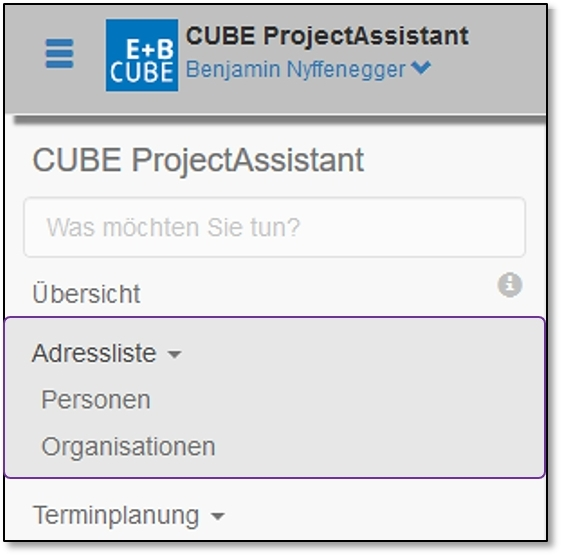
\includegraphics[width=1\linewidth]{../chapters/03_Adressliste/pictures/3-1_Menu_Adressliste.jpg}
  \end{center}
  \vspace{-20pt}
  \caption{Die Adressliste verwenden}
  \vspace{-10pt}
\end{wrapfigure}

Wählen Sie aus dem Menü links den Punkt 'Adressliste' aus.

\vspace{7cm}

Es erscheint eine Liste mit sämtlichen im CUBE PA hinterlegten Adressen von Personen und Firmen:

\begin{figure}[H]
\center{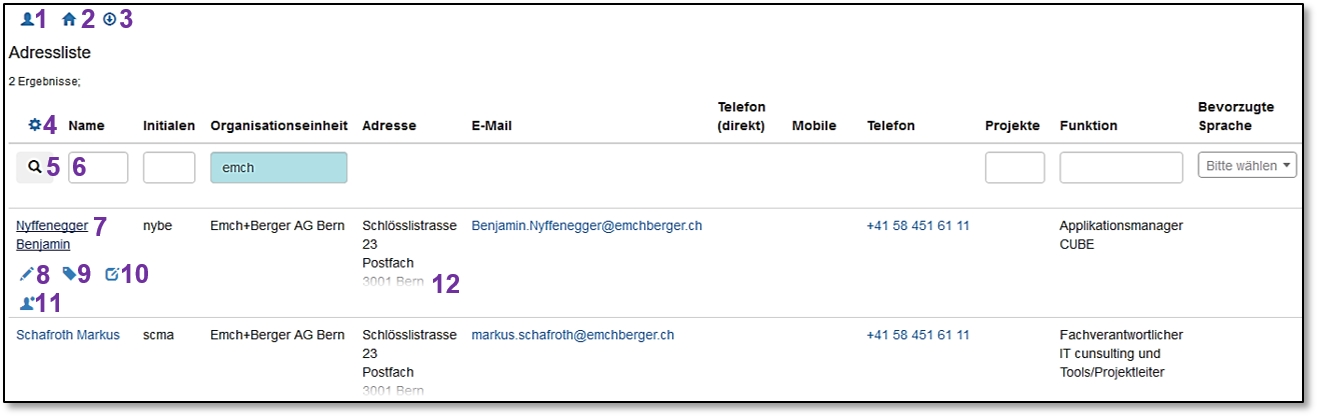
\includegraphics[width=1\linewidth]{../chapters/03_Adressliste/pictures/3-1_Adressliste_Uebersicht.jpg}}
\caption{Die Übersicht der Adressliste}
% \label{fig:speciation}
\end{figure}

Oben links haben Sie die Möglichkeit, neue Personen 
\includegraphics[height=12pt]{/Icons/Person.jpg} oder Firmen 
\includegraphics[height=12pt]{/Icons/Haus.jpg} zu erfassen. Beachten Sie die Eigenschaften, welche eingangs des Kapitels aufgeführt wurden (Kapitel \ref{bkm:Ref443738751}). \newline
Für die Suche / Filterung von Einträgen stehen Ihnen zwei Felder zur Verfügung. Geben Sie im Feld 'Name' und/oder 'Organisationseinheit' \col{(3)} einen Suchbegriff ein und klicken Sie mit der Maus auf das Lupensymbol 
\includegraphics[height=12pt]{/Icons/Lupe_kl.jpg} \col{(4)} oder betätigen Sie die 'Enter'-Taste. Alle gefunden Einträge werden angezeigt. Mit Klick auf das Kreuzchen \col{(5)} können Sie sämtliche Filtereinträge zurücksetzen. \newline
Sie haben die Möglichkeit eine vCard (Adresskarte z.B. für Outlook) herunterzuladen. Klicken Sie auf das vCard-Symbol 
\includegraphics[height=12pt]{/Icons/vCard.jpg} \col{6)}. Sie werden anschliessend gefragt, ob Sie die vCard öffnen
oder speichern wollen.\newline
Mit Klick auf die E-Mail-Adresse \col{(7)} haben Sie die Möglichkeit, der ausgewählten Person eine E-Mail zu schreiben. Ein Klick auf die Telefonnummer \col{(8)} ermöglicht die Person z.B. mittels Skype anzurufen (Abhängig von der Installation).\newline
Wenn Sie auf das Bearbeitungssymbol 
\includegraphics[height=12pt]{/Icons/Bearbeiten.jpg} \col{(9)} klicken, können Sie die Einträge einer Person oder Firma ändern. Dazu benötigen Sie jedoch die erforderlichen Zugriffsrechte. Mit Klick auf das Stiftsymbol 
\includegraphics[height=12pt]{/Icons/Stift.jpg} \col{(10)} gelangen Sie direkt zu den Benutzereinstellungen (im Menü Benutzerverwaltung). Auch hierzu benötigen Sie die entsprechenden Berechtigungen, damit Sie Änderungen vornehmen können.

\subsection{Neue Personen oder Firmen in der Adressliste erfassen}
\label{bkm:Ref2018071901}
Berechtigte Benutzer können in der Adressliste neue Personen oder Firmen erfassen oder bestehende Einträge ändern:

\vspace{\baselineskip}

\begin{tabular}{cc} %{cl}
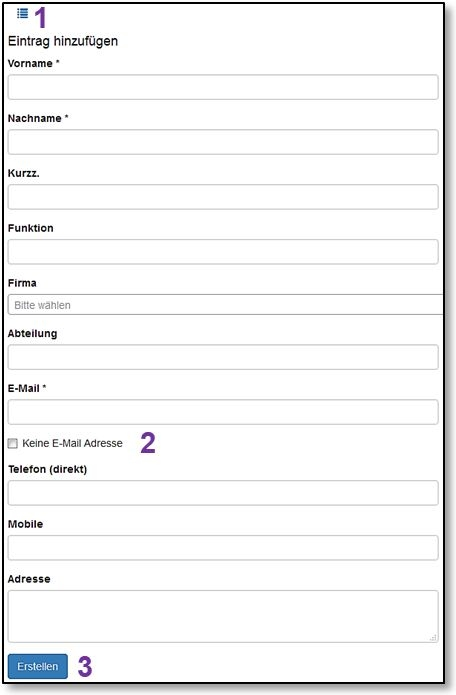
\includegraphics[width=0.49\textwidth]{../chapters/03_Adressliste/pictures/3-2_Personeneintraege.jpg} & 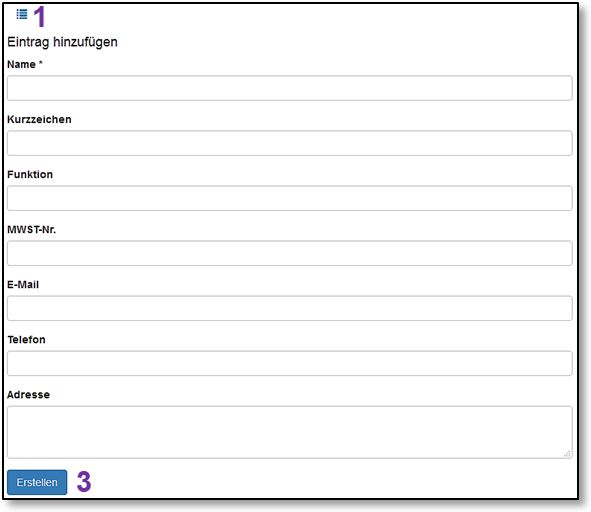
\includegraphics[width=0.49\textwidth]{../chapters/03_Adressliste/pictures/3-2_Firmeneintraege.jpg} \\
Personeneinträge & Firmeneinträge \\
\end{tabular}

% \begin{figure} 
%      \subfigure{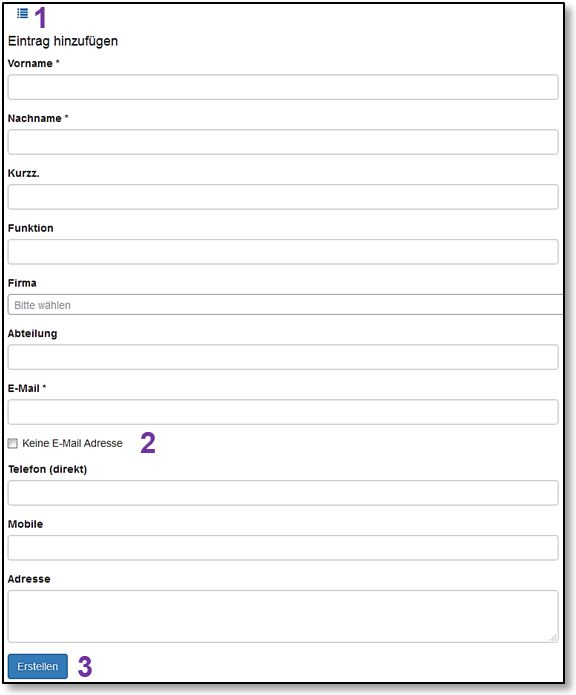
\includegraphics[width=0.49\textwidth]{32_Personeneintraege.jpg}} 
%      \subfigure{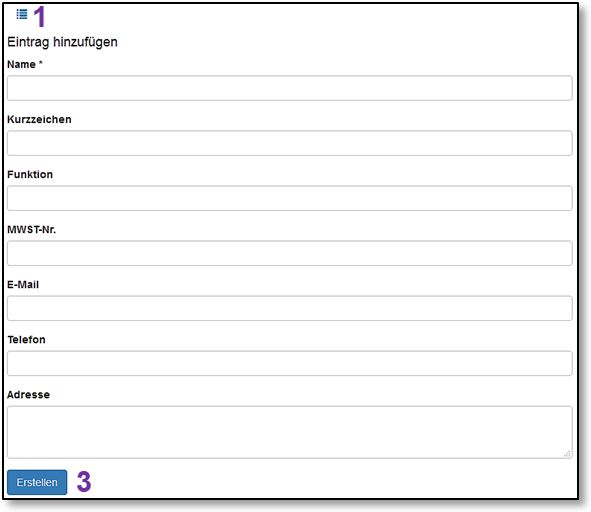
\includegraphics[width=0.49\textwidth]{32_Firmeneintraege.jpg}} 
% \caption{Die verschiedenen Eingabemasken der Adressliste} 
% \end{figure}

\vspace{\baselineskip}
Alle Felder mit * sind Pflichtfelder und müssen ausgefüllt werden. Kann / soll keine E-Mail-Adresse hinterlegt werden, kann dieses Pflichtfeld mittels einem Häkchen 'Keine E-Mail-Adresse' \col{(2)} umgangen und leergelassen werden. Nach dem Eingeben der gewünschten / bekannten Feldern wird der Datensatz mit 'Erstellen' \col{(3)} gespeichert und steht anschliessend in der Adressliste zur Verfügung. Wurde bei einem bestehenden Eintrag auf das Bearbeitungssymbol 
\includegraphics[height=12pt]{/Icons/Bearbeiten.jpg} geklickt, wird die gleiche Maske (siehe oben) geöffnet. Alle bereits hinterlegten Daten sind in den entsprechenden Feldern vorhanden und können geändert werden. Wie oben eingangs des Kapitels bereits vermerkt, kann bei einer Person die Firmenzugehörigkeit aus Sicherheitsgründen (Zugriffsrechte) nicht, resp. nur durch den Administrator geändert werden.\newline
Durch Klick auf das Listensymbol 
\includegraphics[height=12pt]{/Icons/Listensymbol_zurueck.jpg} \col{(1)} gelangen Sie zurück zur Adressliste.
